\documentclass[11pt]{article}
\usepackage{amsmath}
\usepackage{geometry}                % See geometry.pdf to learn the layout options. There are lots.
\geometry{letterpaper}                   % ... or a4paper or a5paper or ... 
%\geometry{landscape}                % Activate for for rotated page geometry
%\usepackage[parfill]{parskip}    % Activate to begin paragraphs with an empty line rather than an indent
\usepackage{graphicx}
\usepackage{amssymb}
\usepackage{epstopdf}
\DeclareGraphicsRule{.tif}{png}{.png}{`convert #1 `dirname #1`/`basename #1 .tif`.png}

%Don't list section numbers
\setcounter{secnumdepth}{0}

\title{CS 1653: Applied Cryptography and Network Security\\Term Project, Phase 4}
\author{Lindsey ``Hellman" Bieda\quad\texttt{leb35@pitt.edu}\\Tucker ``Diffie" Trainor\quad\texttt{tmt33@pitt.edu}}
\date{April 5, 2012} % Activate to display a given date or no date

\begin{document}
\maketitle
\section{Introduction: Cryptographic Techniques}
(an introductory paragraph or two that broadly surveys the types of cryptographic techniques that your group has decided to use to address threats T5-T7)
% Threat 5
\section{Threat 5: Message Reorder, Replay, or Modification}
\subsection{Threat Description}
Begin by describing the threat treated in this section. This may include describing examples of the threat being exploited by an adversary, a short discussion of why this threat is problematic and needs to be addressed, and/or diagrams showing how the threat might manifest in your group�s current implementation.
\subsection{Mechanism Description}
The mechanism builds upon the protocols used in Threats 1-4 that establish a secure session key between a client and a server. Though messages passed in the session are secure from eavesdropping, they are not secure from reorder, replay, or modification. We use two methods to eliminate these new threats: sequence numbers and message authentication.

Sequence numbers are a simple yet effective tool that would alert either end of channel that a message has ben reordered or replayed. We modify our message format so that it includes an integer field to store the sequence number. Then, after receiving a message, the receiving party increments the sequence number by 1 and uses that value in their response. Replays and reordering of messages are easily detectable by either party, as the sequence number will reveal an inconsistency.

Message authentication is a cryptographic principal that is used to verify that a message has not been tampered with.
\begin{figure}[htbp]
\begin{center}
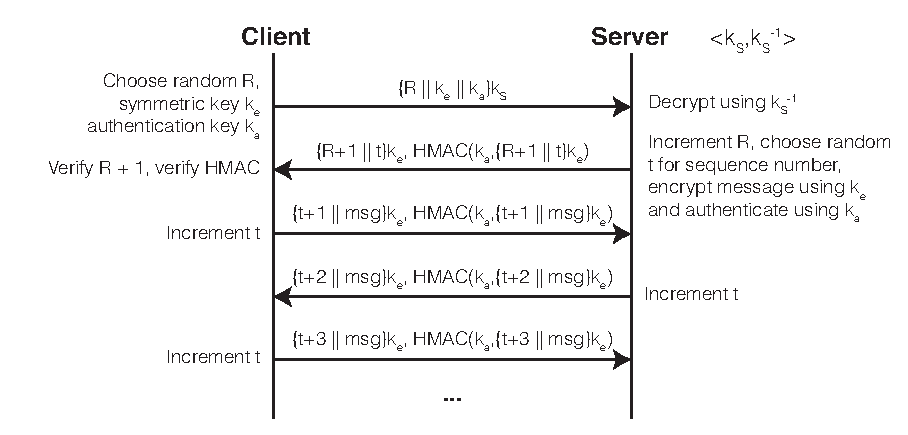
\includegraphics{threat5.eps}
\caption{Threat 5 Mechanism}
\label{threat5}
\end{center}
\end{figure}
\subsection{Correctness and Security of Mechanism}
Lastly, provide a short argument addressing why your proposed mechanism sufficiently addresses this particular threat. This argument should address the correctness of your approach, as well as its overall security. For example, if your mechanism involves a key agreement or key exchange protocol, you should argue that both parties agree on the same key (correctness) and that no other party can figure out the key (security).
% Threat 6
\section{Threat 6: File Leakage}
\subsection{Threat Description}
Begin by describing the threat treated in this section. This may include describing examples of the threat being exploited by an adversary, a short discussion of why this threat is problematic and needs to be addressed, and/or diagrams showing how the threat might manifest in your group�s current implementation.
\subsection{Mechanism Description}
Next, provide a short description of the mechanism that you chose to implement to protect against this threat. For interactive protocols, it would be helpful to provide a diagram explaining the messages exchanged between participating principals. (See the notes from Lecture 10 for example diagrams.) Be sure to explain any cryptographic choices that your group makes: What types of algorithms, modes of operation, and/or key lengths did you chose? Why? If shared keys are needed, how are they exchanged?
\begin{figure}[htbp]
\begin{center}
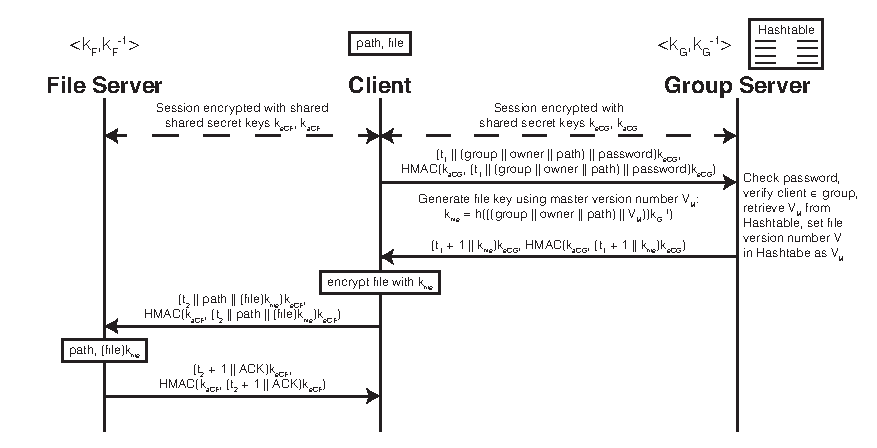
\includegraphics{threat6a.eps}
\caption{Threat 6 Mechanism: Hashtable and Operations}
\label{threat6a}
\end{center}
\end{figure}
%\begin{figure}[htbp]
%\begin{center}
%\includegraphics{threat6b.eps}
%\caption{Threat 6 Mechanism: Diagram}
%\label{threat6b}
%\end{center}
%\end{figure}
\subsection{Correctness and Security of Mechanism}
Lastly, provide a short argument addressing why your proposed mechanism sufficiently addresses this particular threat. This argument should address the correctness of your approach, as well as its overall security. For example, if your mechanism involves a key agreement or key exchange protocol, you should argue that both parties agree on the same key (correctness) and that no other party can figure out the key (security).
% Threat 7
\section{Threat 7: Token Theft}
\subsection{Threat Description}
stub
\subsection{Mechanism Description}
stub
\begin{figure}[htbp]
\begin{center}
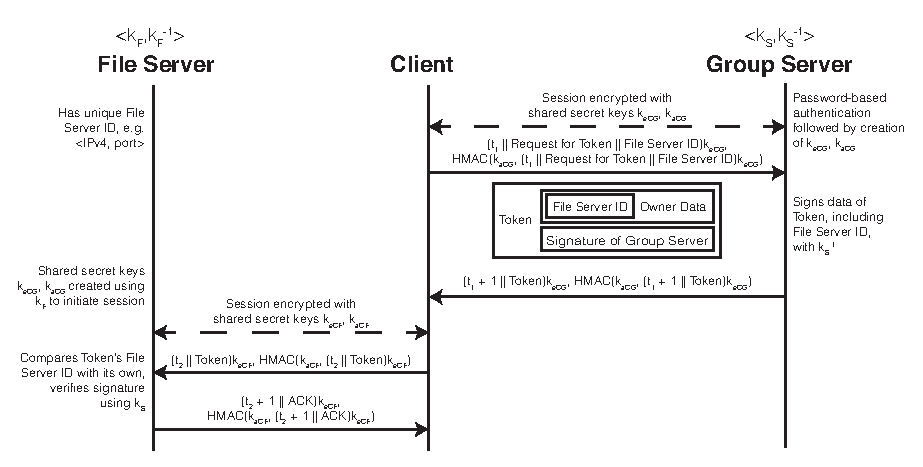
\includegraphics{threat7.eps}
\caption{Threat 7 Mechanism}
\label{threat7}
\end{center}
\end{figure}
\subsection{Correctness and Security of Mechanism}
stub
\section{Discussion and Commentary}
After completing one section for each threat, conclude with a paragraph or two discussing the interplay between your proposed mechanisms, and commenting on the design process that your group followed. Did you discuss other ideas that didn�t pan out before settling on the above-documented approach? Did you end up designing a really interesting protocol suite that addresses multiple threats at once? Use this space to show off your hard work!
\section{Threats 1 through 4 revisited}
Finally, spend about one paragraph convincing me that your modified protocols still address the threats T1-T4 described in Phase 3 of the project. Full credit for Phase 4 requires that all Phase 3 threats are still protected against.
\end{document}
